% Created by tikzDevice version 0.12.3.1 on 2021-12-15 14:08:26
% !TEX encoding = UTF-8 Unicode
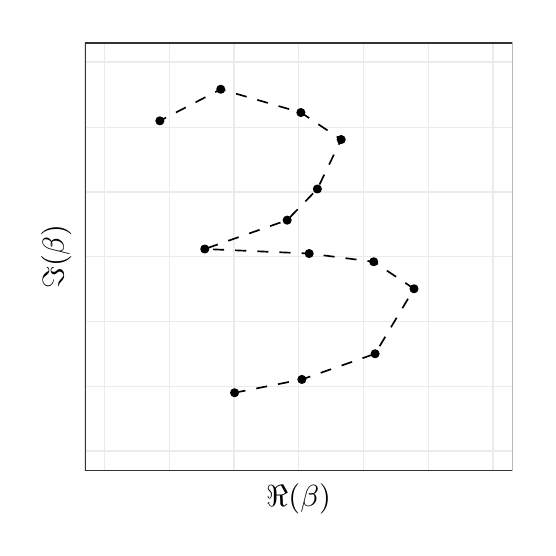
\begin{tikzpicture}[x=1pt,y=1pt]
\definecolor{fillColor}{RGB}{255,255,255}
\path[use as bounding box,fill=fillColor,fill opacity=0.00] (0,0) rectangle (180.67,180.67);
\begin{scope}
\path[clip] (  0.00,  0.00) rectangle (180.67,180.67);
\definecolor{drawColor}{RGB}{255,255,255}
\definecolor{fillColor}{RGB}{255,255,255}

\path[draw=drawColor,line width= 0.6pt,line join=round,line cap=round,fill=fillColor] (  0.00,  0.00) rectangle (180.67,180.68);
\end{scope}
\begin{scope}
\path[clip] ( 20.71, 20.71) rectangle (175.17,175.17);
\definecolor{fillColor}{RGB}{255,255,255}

\path[fill=fillColor] ( 20.71, 20.71) rectangle (175.17,175.17);
\definecolor{drawColor}{gray}{0.92}

\path[draw=drawColor,line width= 0.3pt,line join=round] ( 20.71, 51.14) --
	(175.17, 51.14);

\path[draw=drawColor,line width= 0.3pt,line join=round] ( 20.71, 97.94) --
	(175.17, 97.94);

\path[draw=drawColor,line width= 0.3pt,line join=round] ( 20.71,144.75) --
	(175.17,144.75);

\path[draw=drawColor,line width= 0.3pt,line join=round] ( 51.14, 20.71) --
	( 51.14,175.17);

\path[draw=drawColor,line width= 0.3pt,line join=round] ( 97.94, 20.71) --
	( 97.94,175.17);

\path[draw=drawColor,line width= 0.3pt,line join=round] (144.75, 20.71) --
	(144.75,175.17);

\path[draw=drawColor,line width= 0.6pt,line join=round] ( 20.71, 27.74) --
	(175.17, 27.74);

\path[draw=drawColor,line width= 0.6pt,line join=round] ( 20.71, 74.54) --
	(175.17, 74.54);

\path[draw=drawColor,line width= 0.6pt,line join=round] ( 20.71,121.35) --
	(175.17,121.35);

\path[draw=drawColor,line width= 0.6pt,line join=round] ( 20.71,168.15) --
	(175.17,168.15);

\path[draw=drawColor,line width= 0.6pt,line join=round] ( 27.74, 20.71) --
	( 27.74,175.17);

\path[draw=drawColor,line width= 0.6pt,line join=round] ( 74.54, 20.71) --
	( 74.54,175.17);

\path[draw=drawColor,line width= 0.6pt,line join=round] (121.35, 20.71) --
	(121.35,175.17);

\path[draw=drawColor,line width= 0.6pt,line join=round] (168.15, 20.71) --
	(168.15,175.17);
\definecolor{drawColor}{RGB}{0,0,0}

\path[draw=drawColor,line width= 0.6pt,dash pattern=on 4pt off 4pt ,line join=round] ( 74.76, 48.75) --
	( 99.08, 53.56) --
	(125.54, 62.83) --
	(139.60, 86.32) --
	(125.04, 96.08) --
	(101.71, 99.05) --
	( 63.99,100.69) --
	( 93.77,111.12) --
	(104.68,122.37) --
	(113.28,140.24) --
	( 98.72,150.00) --
	( 69.76,158.42) --
	( 47.77,147.00);
\definecolor{fillColor}{RGB}{0,0,0}

\path[draw=drawColor,line width= 0.4pt,line join=round,line cap=round,fill=fillColor] ( 74.76, 48.75) circle (  1.43);

\path[draw=drawColor,line width= 0.4pt,line join=round,line cap=round,fill=fillColor] ( 99.08, 53.56) circle (  1.43);

\path[draw=drawColor,line width= 0.4pt,line join=round,line cap=round,fill=fillColor] (125.54, 62.83) circle (  1.43);

\path[draw=drawColor,line width= 0.4pt,line join=round,line cap=round,fill=fillColor] (139.60, 86.32) circle (  1.43);

\path[draw=drawColor,line width= 0.4pt,line join=round,line cap=round,fill=fillColor] (125.04, 96.08) circle (  1.43);

\path[draw=drawColor,line width= 0.4pt,line join=round,line cap=round,fill=fillColor] (101.71, 99.05) circle (  1.43);

\path[draw=drawColor,line width= 0.4pt,line join=round,line cap=round,fill=fillColor] ( 63.99,100.69) circle (  1.43);

\path[draw=drawColor,line width= 0.4pt,line join=round,line cap=round,fill=fillColor] ( 93.77,111.12) circle (  1.43);

\path[draw=drawColor,line width= 0.4pt,line join=round,line cap=round,fill=fillColor] (104.68,122.37) circle (  1.43);

\path[draw=drawColor,line width= 0.4pt,line join=round,line cap=round,fill=fillColor] (113.28,140.24) circle (  1.43);

\path[draw=drawColor,line width= 0.4pt,line join=round,line cap=round,fill=fillColor] ( 98.72,150.00) circle (  1.43);

\path[draw=drawColor,line width= 0.4pt,line join=round,line cap=round,fill=fillColor] ( 69.76,158.42) circle (  1.43);

\path[draw=drawColor,line width= 0.4pt,line join=round,line cap=round,fill=fillColor] ( 47.77,147.00) circle (  1.43);
\definecolor{drawColor}{gray}{0.20}

\path[draw=drawColor,line width= 0.6pt,line join=round,line cap=round] ( 20.71, 20.71) rectangle (175.17,175.17);
\end{scope}
\begin{scope}
\path[clip] (  0.00,  0.00) rectangle (180.67,180.67);
\definecolor{drawColor}{RGB}{0,0,0}

\node[text=drawColor,anchor=base,inner sep=0pt, outer sep=0pt, scale=  1.10] at ( 97.94,  7.64) {$\Re(\beta)$};
\end{scope}
\begin{scope}
\path[clip] (  0.00,  0.00) rectangle (180.67,180.67);
\definecolor{drawColor}{RGB}{0,0,0}

\node[text=drawColor,rotate= 90.00,anchor=base,inner sep=0pt, outer sep=0pt, scale=  1.10] at ( 13.08, 97.94) {$\Im(\beta)$};
\end{scope}
\end{tikzpicture}
